\documentclass[10pt,a4paper]{article}
\usepackage[utf8]{inputenc}
\usepackage[english]{babel}
\usepackage[T1]{fontenc}
\usepackage{amsmath}
\usepackage{amsfonts}
\usepackage{amssymb}
\usepackage{lmodern}
\usepackage{fancyvrb}
\usepackage{tikz}
\usepackage{verbatim}
\usepackage{indentfirst}
\usepackage{hyperref}
\hypersetup{
    colorlinks=true,
    linkcolor=blue, % Couleur des liens internes
    citecolor=red, % Couleur des numéros de la biblio dans le corps
    urlcolor=blue} % Couleur des url

\newcommand{\version}{\IfFileExists{../../version.txt}
{\input{../../version.txt}}
{\input{../../../version.txt}}
}

\newcommand{\command}[1]{%
\indent \fcolorbox{black}{white}{%
   \begin{minipage}{\dimexpr\textwidth-\parindent\relax}%
      #1
   \end{minipage}%
}
}

\newsavebox{\FVerbBox}
\newenvironment{sample}
{\par \vspace{0.2cm} \begin{lrbox}{\FVerbBox}
\begin{minipage}{\dimexpr\textwidth-\parindent\relax}}
{\end{minipage}
\end{lrbox}
\fcolorbox{black}{lightgray}{\usebox{\FVerbBox}}
\vspace{0.2cm}}

\newenvironment{sampletitle}
{\vspace{0.2cm} \noindent\textbf{Example} :
\begin{sample}}
{\end{sample}}

\newcommand{\samplecomment}[1]{%

\textit{#1}
}

\newcommand{\seealso}[1]{\vspace{0.2cm} \noindent\textbf{See also} :\par #1}

% tikz
\usetikzlibrary{calc}
\usetikzlibrary{arrows}
\usetikzlibrary{shadows}

\tikzset{block/.style={draw, text centered, fill=gray!10,drop shadow}}
\tikzset{connect/.style={draw, line width=1 pt}}

\author{Sebastien CAUX}
\title{\tool{} reference documentation \version \\ \gpprocdevice{(since v0.95)} \gpcomp{since v1.02}}

\begin{document}
\maketitle
\section{Introduction}
\tool{} is a command line tool that allows to create new \kind{} block.

\section{Use}
\tool{} always takes the \kind{} file in the current directory, so you only can have one \kind{} definition per directory. A \kind{} file have the `\ext{}' extension.

At the beginning, you need to create a \kind{} with the \emph{new} command. After that, you can use all the commands set on this \kind{}.

Refer to the tutorial `GPStudio command line quick start' to learn how to use this tool.

Under linux, you have a completion script to help you writing commands.

\section{Commands}
% ==============================================
\subsection{brief}
The commands of this tools are used to define inputs and outputs of the block, flows, Parameter Interconnect interface with internal registers, \gpdevice{external ports, }clocks and resets. Finally, high level properties for the controller of the block can be specified.

\gpcomp{
\begin{figure}[h!]
\centering
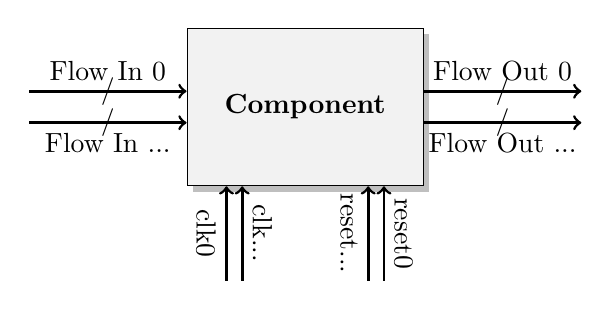
\begin{tikzpicture}
\node[block,rectangle,minimum height=2cm,minimum width=3cm] (bloc) {\textbf{Component}};

\path[connect,<-] ([yshift=0.2cm]bloc.west) -- node{/} node[above]{Flow In 0} ++(-2cm,0);
\path[connect,<-] ([yshift=-0.2cm]bloc.west) -- node{/} node[below]{Flow In ...} ++(-2cm,0);

\path[connect,->] ([yshift=0.2cm]bloc.east) -- node{/} node[above]{Flow Out 0} ++(2cm,0);
\path[connect,->] ([yshift=-0.2cm]bloc.east) -- node{/} node[below]{Flow Out ...} ++(2cm,0);

\path[connect,<-] ([xshift=-1cm]bloc.south) -- node[sloped,below]{clk0} ++(0,-1.2cm);
\path[connect,<-] ([xshift=-0.8cm]bloc.south) -- node[sloped,above]{clk...} ++(0,-1.2cm);

\path[connect,<-] ([xshift=1cm]bloc.south) -- node[sloped,above]{reset0} ++(0,-1.2cm);
\path[connect,<-] ([xshift=0.8cm]bloc.south) -- node[sloped,below]{reset...} ++(0,-1.2cm);
\end{tikzpicture}
\caption{Component block}
\end{figure}
}
\gpproc{
\begin{figure}[h!]
\centering
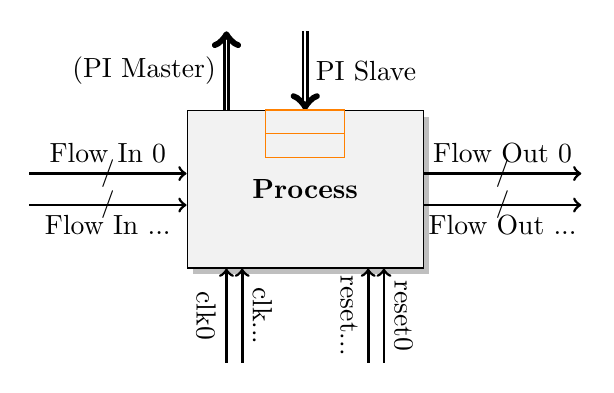
\begin{tikzpicture}
\node[block,rectangle,minimum height=2cm,minimum width=3cm] (bloc) {\textbf{Process}};

\path[connect,<-] ([yshift=0.2cm]bloc.west) -- node{/} node[above]{Flow In 0} ++(-2cm,0);
\path[connect,<-] ([yshift=-0.2cm]bloc.west) -- node{/} node[below]{Flow In ...} ++(-2cm,0);

\path[connect,->] ([yshift=0.2cm]bloc.east) -- node{/} node[above]{Flow Out 0} ++(2cm,0);
\path[connect,->] ([yshift=-0.2cm]bloc.east) -- node{/} node[below]{Flow Out ...} ++(2cm,0);

\path[connect,<-,double] (bloc.north) -- node[right]{PI Slave} ++(0,1cm);
\path[connect,->,double] ([xshift=-1cm]bloc.north) -- node[left]{(PI Master)} ++(0,1cm);

\draw[color=orange] ([xshift=-0.5cm]bloc.north) rectangle ([xshift=0.5cm,yshift=-0.3cm]bloc.north);
\draw[color=orange] ([xshift=-0.5cm,yshift=-0.3cm]bloc.north) rectangle ([xshift=0.5cm,yshift=-0.6cm]bloc.north);

\path[connect,<-] ([xshift=-1cm]bloc.south) -- node[sloped,below]{clk0} ++(0,-1.2cm);
\path[connect,<-] ([xshift=-0.8cm]bloc.south) -- node[sloped,above]{clk...} ++(0,-1.2cm);

\path[connect,<-] ([xshift=1cm]bloc.south) -- node[sloped,above]{reset0} ++(0,-1.2cm);
\path[connect,<-] ([xshift=0.8cm]bloc.south) -- node[sloped,below]{reset...} ++(0,-1.2cm);
\end{tikzpicture}
\caption{Process block}
\end{figure}
}
\gpdevice{
\begin{figure}[h!]
\centering
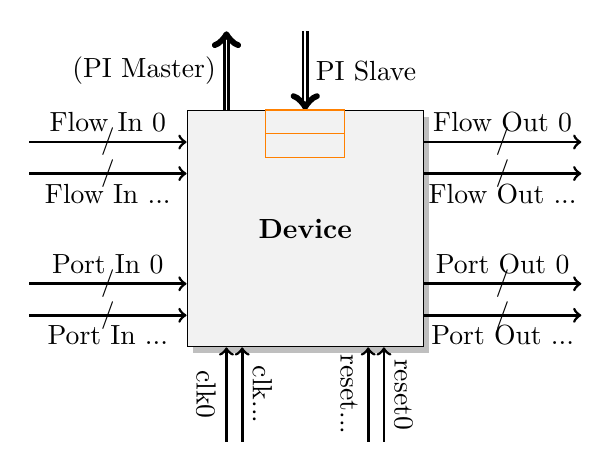
\begin{tikzpicture}
\node[block,rectangle,minimum height=3cm,minimum width=3cm] (bloc) {\textbf{Device}};

\path[connect,<-] ([yshift=1.1cm]bloc.west) -- node{/} node[above]{Flow In 0} ++(-2cm,0);
\path[connect,<-] ([yshift=0.7cm]bloc.west) -- node{/} node[below]{Flow In ...} ++(-2cm,0);

\path[connect,<-] ([yshift=-0.7cm]bloc.west) -- node{/} node[above]{Port In 0} ++(-2cm,0);
\path[connect,<-] ([yshift=-1.1cm]bloc.west) -- node{/} node[below]{Port In ...} ++(-2cm,0);

\path[connect,->] ([yshift=1.1cm]bloc.east) -- node{/} node[above]{Flow Out 0} ++(2cm,0);
\path[connect,->] ([yshift=0.7cm]bloc.east) -- node{/} node[below]{Flow Out ...} ++(2cm,0);

\path[connect,->] ([yshift=-0.7cm]bloc.east) -- node{/} node[above]{Port Out 0} ++(2cm,0);
\path[connect,->] ([yshift=-1.1cm]bloc.east) -- node{/} node[below]{Port Out ...} ++(2cm,0);

\path[connect,<-,double] (bloc.north) -- node[right]{PI Slave} ++(0,1cm);
\path[connect,->,double] ([xshift=-1cm]bloc.north) -- node[left]{(PI Master)} ++(0,1cm);

\draw[color=orange] ([xshift=-0.5cm]bloc.north) rectangle ([xshift=0.5cm,yshift=-0.3cm]bloc.north);
\draw[color=orange] ([xshift=-0.5cm,yshift=-0.3cm]bloc.north) rectangle ([xshift=0.5cm,yshift=-0.6cm]bloc.north);

\path[connect,<-] ([xshift=-1cm]bloc.south) -- node[sloped,below]{clk0} ++(0,-1.2cm);
\path[connect,<-] ([xshift=-0.8cm]bloc.south) -- node[sloped,above]{clk...} ++(0,-1.2cm);

\path[connect,<-] ([xshift=1cm]bloc.south) -- node[sloped,above]{reset0} ++(0,-1.2cm);
\path[connect,<-] ([xshift=0.8cm]bloc.south) -- node[sloped,below]{reset...} ++(0,-1.2cm);
\end{tikzpicture}
\caption{Device block}
\end{figure}
}

Commands of \tool{} always have the same naming convention. This table is a brief commands list depending on the model instance to be modified.\\

\noindent\begin{tabular}{|c|c|c|c|c|c|}
\hline 
 & \textbf{add} & \textbf{del} & \textbf{show} & \textbf{rename} & \textbf{set} \\ 
\hline 
\textbf{file} & \hyperref[subsec:addfile]{addfile} & \hyperref[subsec:delfile]{delfile} & \hyperref[subsec:showfile]{showfile} &  &  \\ 
\hline 
\textbf{flow} & \hyperref[subsec:addflow]{addflow} & \hyperref[subsec:delflow]{delflow} & \hyperref[subsec:showflow]{showflow} & \hyperref[subsec:renameflow]{renameflow} & \hyperref[subsec:setflow]{setflow}  \\ 
\hline 
\textbf{param} & \hyperref[subsec:addparam]{addparam} & \hyperref[subsec:delparam]{delparam} & \hyperref[subsec:showparam]{showparam} & \hyperref[subsec:renameparam]{renameparam} & \hyperref[subsec:setparam]{setparam}  \\ 
\hline 
\gpprocdevice{
\textbf{bitfield} & \hyperref[subsec:addbitfield]{addbitfield} & \hyperref[subsec:delbitfield]{delbitfield} & \hyperref[subsec:showbitfield]{showbitfield} & \hyperref[subsec:renamebitfield]{renamebitfield} & \hyperref[subsec:setbitfield]{setbitfield}  \\ 
\hline 
\textbf{property} & \hyperref[subsec:addproperty]{addproperty} & \hyperref[subsec:delproperty]{delproperty} & \hyperref[subsec:showproperty]{showproperty} & \hyperref[subsec:renameproperty]{renameproperty} & \hyperref[subsec:setproperty]{setproperty}  \\ 
\hline 
\textbf{enum} & \hyperref[subsec:addenum]{addenum} & \hyperref[subsec:delenum]{delenum} & \hyperref[subsec:showenum]{showenum} &  &  \\ 
\hline 
}
\textbf{reset} & \hyperref[subsec:addreset]{addreset} & \hyperref[subsec:delreset]{delreset} & \hyperref[subsec:showreset]{showreset} & \hyperref[subsec:renamereset]{renamereset} & \hyperref[subsec:setreset]{setreset}  \\ 
\hline 
\textbf{clock} & \hyperref[subsec:addclock]{addclock} & \hyperref[subsec:delclock]{delclock} & \hyperref[subsec:showclock]{showclock} & \hyperref[subsec:renameclock]{renameclock} & \hyperref[subsec:setclock]{setclock}  \\ 
\hline 
\gpdevice{
\textbf{extport} & \hyperref[subsec:addextport]{addextport} & \hyperref[subsec:delextport]{delextport} & \hyperref[subsec:showextport]{showextport} &  &   \\ 
\hline 
}
\end{tabular}\\

Few over commands can be used to create the block and generate the skeleton defined in project section. The command \hyperref[subsec:sethelp]{sethelp} is useful to document the block. In addition, \hyperref[subsec:setinfo]{setinfo} saves the informations about the block.

\hyperref[subsec:setpropertymap]{setpropertymap} defines link between properties.

For Parameters Interconnect interface configuration, you should use \hyperref[subsec:setpisizeaddr]{setpisizeaddr} and \hyperref[subsec:setpimastercount]{setpimastercount}.

\subsection{project}
% ==============================================
\gpproc{
\subsubsection{new}
\command{\textbf{\tool{} new} -n <\kind{}-name>}

Creates a \kind{} file inside the current directory named `\texttt{<\kind{}-name>}.proc'.\\

\paramcommand{
-n & \kind{} name without space & my\_\kind{} \\ 
}

\begin{sampletitle}
> \textbf{\tool{} new\kind{}} -n my\_\kind{}
\end{sampletitle}
\samplecomment{Creates a new \kind{} named \texttt{my\_\kind{}}. After that, you have a file project \texttt{my\_\kind{}.proc} in the current directory.}
}

% ==============================================
\gpdevice{
\subsubsection{new}
\command{\textbf{\tool{} new} -n <\kind{}-name>}

Creates a \kind{} file inside the current directory named `\texttt{<\kind{}-name>}.\kind{}' to define a new custom \kind{} driver support.\\

\paramcommand{
-n & \kind{} name without space & my\_\kind{} \\ 
}

\begin{sampletitle}
> \textbf{\tool{} new} -n my\_\kind{}
\end{sampletitle}
\samplecomment{Creates a new \kind{} named \texttt{my\_\kind{}}. After that, you have a file project \texttt{my\_\kind{}.io} in the current directory.}
}
% ==============================================
\subsubsection{showblock}
\command{\textbf{\tool{} showblock}}

Shows all informations about the block.

% ==============================================
\subsubsection{generatetop}
\command{\textbf{\tool{} generatetop} [-o <dir>]}

Generates the skeleton of the block top level in the subdirectory \texttt{build/}. This top level instantiate the \kind{} and the slave if you need. The generated file is named `<\kind{}-name>.vhd'.\\

\paramcommand{
-o & output directory & build \\ 
}

\begin{sampletitle}
> \textbf{\tool{} generatetop} -o build/
\end{sampletitle}
\samplecomment{Generates \texttt{myproc.vhd} in the subdirectory \texttt{build/}.}

% ==============================================
\subsubsection{generateslave}
\command{\textbf{\tool{} generateslave} [-o <dir>]}

Generates the slave for dynamic parameters with read and write. The generated file is named `<\kind{}-name>\_slave.vhd'.\\

\paramcommand{
-o & output directory & build \\ 
}

\begin{sampletitle}
> \textbf{\tool{} generateslave} -o build/
\end{sampletitle}
\samplecomment{Generates \texttt{myproc\_slave.vhd} in the subdirectory \texttt{build/}.}

% ==============================================
\subsubsection{generateprocess}
\command{\textbf{\tool{} generateprocess} [-o <dir>]}

Generates an empty skeleton to implement your custom \kind{}. The generated file is named `<\kind{}-name>\_process.vhd'.\\

\paramcommand{
-o & output directory & build \\ 
}

\begin{sampletitle}
> \textbf{\tool{} generateprocess} -o build/
\end{sampletitle}
\samplecomment{Generates \texttt{myproc\_process.vhd} in the subdirectory \texttt{build/}.}

% ==============================================
\subsubsection{generate}
\command{\textbf{\tool{} generate} [-o <dir>]}

This command is an alias for the three previous command. Generates all the three files.\\

\paramcommand{
-o & output directory & build \\ 
}

\begin{sampletitle}
> \textbf{\tool{} generate} -o build/
\end{sampletitle}
\samplecomment{Generates \texttt{myproc.vhd}, \texttt{myproc\_process.vhd} and \texttt{myproc\_slave.vhd} in the subdirectory \texttt{build/}.}

% ==============================================
\subsubsection{generatetb}
\command{\textbf{\tool{} generatetb} [-o <dir>]}

Generates a testbench that implement your \kind{}. This generated test bench simulates clocks and resets and sends stimuli file named `<flow-name>.stim` for each input flows and saves output data to `<flow-name>.data`. To obtain stim file and retrieve data from data file you should use \textbf{convert}.\\

\paramcommand{
-o & output directory & build \\ 
}

\begin{sampletitle}
> \textbf{\tool{} generatetb} -o build/
\end{sampletitle}
\samplecomment{Generates \texttt{myproc\_tb.vhd} in the subdirectory \texttt{build/}.}

\seealso{\textbf{\tool{} convert}}

% ==============================================
\subsubsection{convert}
\command{\textbf{\tool{} convert} -i <input-file> [-o <output-file>]}

Converts file for test bench purpose. Can convert picture files to stim file or data files to picture files.\\

\paramcommand{
-i & input file & img1.png \newline out.data \\ 
\hline
-o & output file & in.stim \newline out.jpg \\ 
}

\begin{sampletitle}[1]
> \textbf{\tool{} convert} -i imgage.gif -o in.stim
\end{sampletitle}
\samplecomment{Transforms this gif picture into stimuli file to send to in flow}

\begin{sampletitle}[2]
> \textbf{\tool{} convert} -i out.data -o out.png
\end{sampletitle}
\samplecomment{Transforms the output of the flow `out` to a png image}

\subsection{files}
% ==============================================
\subsubsection{addfile}
\label{subsec:addfile}
\command{\textbf{\tool{} addfile} -p <path> -t <type> -g <group>}

Adds the file with the path \texttt{<path>} to the list of files of the current \kind{} block. The type and group of the file depends of the tool-chain that you use. If the file does not exist, prints a warning.\\

\paramcommand{
-p & \kind{} path relative to the file \kind{} & hdl/my\_\kind{}.vhd \\
\hline
-t & type of the file & [vhdl - verilog ...] \\
\hline
-g & group of the file & [hdl - doc ...] \\
}

\begin{sampletitle}
> \textbf{\tool{} addfile} -p hdl/my\_\kind{}.vhd -t vhdl -g hdl
\end{sampletitle}
\samplecomment{Adds the file `my\_\kind{}.vhd' as a file needed by the hdl implementation of the block.}

\seealso{\textbf{\tool{} delfile} and \textbf{\tool{} showfile}}

% ==============================================
\subsubsection{delfile}
\label{subsec:delfile}
\command{\textbf{\tool{} delfile} -p <path>}

Removes the file with the path \texttt{<path>}.\\

\paramcommand{
-p & \kind{} path relative to the file \kind{} & hdl/my\_\kind{}.vhd \\
}

\begin{sampletitle}
> \textbf{\tool{} delfile} -p hdl/my\_\kind{}.vhd
\end{sampletitle}
\samplecomment{Removes the file `my\_\kind{}.vhd'.}

\seealso{\textbf{\tool{} addfile} and \textbf{\tool{} showfile}}

% ==============================================
\subsubsection{showfile}
\label{subsec:showfile}
\command{\textbf{\tool{} showfile}}

Prints the list of files in the current block project.

\subsection{flows}
% ==============================================
\subsubsection{addflow}
\label{subsec:addflow}
\command{\textbf{\tool{} addflow} -n <flow-name> -d <direction> -s <size>}

Adds a flow interface named \texttt{<flow-name>} to the list of flows. You need to specify the direction of the flow (input or output) and the default size.\\

\paramcommand{
-n & name of the flow & in1 \\
\hline
-d & direction of the flow & [in - out] \\
\hline
-s & default size of the flow interface in bit & 9 \\
}

\begin{sampletitle}
> \textbf{\tool{} addflow} -n out0 -d out -s 8
\end{sampletitle}
\samplecomment{Adds a new flow output named `out0' with a default size of 8 bits.}

\seealso{\textbf{\tool{} delflow} and \textbf{\tool{} showflow}}

% ==============================================
\subsubsection{delflow}
\label{subsec:delflow}
\command{\textbf{\tool{} delflow} -n <flow-name>}

Removes the file with the name \texttt{<flow-name>}.\\

\paramcommand{
-n & name of the flow & in1 \\
}

\begin{sampletitle}
> \textbf{\tool{} delflow} -n out0
\end{sampletitle}
\samplecomment{Removes the flow named `out0'.}

\seealso{\textbf{\tool{} addflow} and \textbf{\tool{} showflow}}

% ==============================================
\subsubsection{showflow}
\label{subsec:showflow}
\command{\textbf{\tool{} showflow}}

Prints the list of flows in the current block project.

% ==============================================
\subsubsection{renameflow}
\label{subsec:renameflow}
\command{\textbf{\tool{} renameflow} -n <flow-name> -v <new-name>}

Renames the flow named \texttt{<flow-name>} with the name \texttt{<new-name>}.\\

\paramcommand{
-n & name of the flow & in1 \\
\hline
-v & new name of the flow & in0 \\
}

\begin{sampletitle}
> \textbf{\tool{} renameflow} -n out0 -v out1
\end{sampletitle}
\samplecomment{Renames the flow `out0' to `out1'.}

\seealso{\textbf{\tool{} delflow}}

% ==============================================
\subsubsection{setflow}
\label{subsec:setflow}
\command{\textbf{\tool{} setflow} -n <flow-name> [-d <direction>] [-s <size>]}

Allows to modify one or more flow parameters like the direction or the default size.\\

\paramcommand{
-n & name of the flow & in1 \\
\hline
-d & direction of the flow & [in - out] \\
\hline
-s & default size of the flow interface in bit & 9 \\
}

\begin{sampletitle}
> \textbf{\tool{} setflow} -n out0 -d in \\
> \textbf{\tool{} setflow} -n out0 -s 9
\end{sampletitle}
\samplecomment{Sets the flow `out0' as input and then sets the default size to 9 bits.}

\subsection{params}
% ==============================================
\subsubsection{addparam}
\label{subsec:addparam}
\command{\textbf{\tool{} addparam} -n <param-name> [-t <type>] [-r <relative-address>] [-v <default-value>] [-m <property-map>]}

Adds a param named \texttt{<param-name>} to the list of params.\\

\paramcommand{
-n & name of the param & param0 \\
\hline
-t & type of the param for fixed param & toolchain-type \\
\hline
-r & relative address of the param for dynamic param & 2 \\
\hline
-v & default value of the param & TRUE \newline 1024 \\
\hline
-m & javascript property map expression  & enable.value \newline mode.bits \newline Math.ceil(\newline in.width.value/4)+4 \\
}

\begin{sampletitle}[1]
> \textbf{\tool{} addparam} -n MAX\_LINE\_WIDTH -t INTEGER -v 1280
\end{sampletitle}
\samplecomment{Adds a new fixed param named `MAX\_LINE\_WIDTH' of type INTEGER with a default value of 1280. This example is typically used to define the size of internal buffer when you have to save a complete line of picture in your process.}

\begin{sampletitle}[2]
> \textbf{\tool{} addparam} -n offset\_reg -r 1 -m offset.value
\end{sampletitle}
\samplecomment{Adds a new register named `offset\_reg' with the relative address 1. The value of the register is linked to the value of the property `offset'.}

\seealso{\textbf{\tool{} delparam}, \textbf{\tool{} showparam} and \textbf{\tool{} setpropertymap}}

% ==============================================
\subsubsection{delparam}
\label{subsec:delparam}
\command{\textbf{\tool{} delparam} -n <param-name>}

Removes the param with the name \texttt{<param-name>}.\\

\paramcommand{
-n & name of the param & param0 \\
}

\begin{sampletitle}
> \textbf{\tool{} delparam} -n param0
\end{sampletitle}
\samplecomment{Removes the param named `param0'.}

\seealso{\textbf{\tool{} addparam} and \textbf{\tool{} showparam}}

% ==============================================
\subsubsection{showparam}
\label{subsec:showparam}
\command{\textbf{\tool{} showparam}}

Prints the list of params in the current block project.

% ==============================================
\subsubsection{renameparam}
\label{subsec:renameparam}
\command{\textbf{\tool{} renameparam} -n <param-name> -v <new-name>}

Renames the param named \texttt{<param-name>} with the name \texttt{<new-name>}.\\

\paramcommand{
-n & name of the param & param0 \\
\hline
-v & new name of the param & param1 \\
}

\begin{sampletitle}
> \textbf{\tool{} renameparam} -n param0 -v param1
\end{sampletitle}
\samplecomment{Renames the param `param0' to `param1'.}

\seealso{\textbf{\tool{} delparam}}

% ==============================================
\subsubsection{setparam}
\label{subsec:setparam}
\command{\textbf{\tool{} setparam} -n <param-name> [-t <type>] [-r <relative-address>] [-v <default-value>]}

Allows to modify one or more param parameters like the type, the default value or the relative address.\\

\paramcommand{
-n & name of the param & param0 \\
\hline
-t & type of the param for fixed param & toolchain-type \\
\hline
-r & relative address of the param for dynamic param & 2 \\
\hline
-v & default value of the param & TRUE \\
}

\begin{sampletitle}[1]
> \textbf{\tool{} setparam} -n status -v 1 -r 4 \\
\end{sampletitle}
\samplecomment{Sets the default value of the dynamic param (register) `status' to 1 and sets the relative address to 4.}

\begin{sampletitle}[2]
> \textbf{\tool{} setparam} -n mode -v LINEAR -t Mode \\
\end{sampletitle}
\samplecomment{Sets the type of the generic `mode' to `Mode' with a default value set to `LINEAR'}

% ==============================================
\subsubsection{fixparam}
\command{\textbf{\tool{} fixparam} -n <param-name> -v <true/false>}

Transforms a param to a fixed parameter  if -v is true or a dynamic parameter else.

\begin{sampletitle}
> \textbf{\tool{} fixparam} -n mode -v true \\
\end{sampletitle}
\samplecomment{Sets the parameter `mode' to a fixed parameter, eg generic value for a VHDL backend}

% ==============================================
\subsubsection{setpisizeaddr}
\label{subsec:setpisizeaddr}
\command{\textbf{\tool{} setpisizeaddr} -v <pisizeaddr>}

Sets the width of PI address bus in bits. For example, with the highest address 9 you should use 4 as the pisizeaddr to have a range of 16 addresses.\\

\paramcommand{
-v & width of PI slave address port in bits & 3 \\
}

\begin{sampletitle}
> \textbf{\tool{} setpisizeaddr} -v 5 \\
\end{sampletitle}
\samplecomment{Sets the parameter pisizeaddr to 5 bits to have 32 possible registers}

% ==============================================
\subsubsection{setpimastercount}
\label{subsec:setpimastercount}
\command{\textbf{\tool{} setpimastercount} -v <pimastercount>}

Sets the number of PI master port.\\

\paramcommand{
-v & number of master port & 1 \\
}

\begin{sampletitle}
> \textbf{\tool{} setpimastercount} -v 1 \\
\end{sampletitle}
\samplecomment{Adds a PI master port to the current \kind{}}

\gpprocdevice{
\subsection{bitfields}
% ==============================================
\subsubsection{addbitfield}
\label{subsec:addbitfield}
\command{\textbf{\tool{} addbitfield} -n <param-name.bitfield-name> -b <bitfield> [-m <property-map>]}

Adds a bit field named \texttt{<bitfield-name>} to the param \texttt{<param-name>}.\\

\paramcommand{
-n & name of the bit field composed by the param name, a dot and the bits field name & param.b0 \\
\hline
-b & bits field & 1\newline 8-4 \newline 2,5,10-9 \\
\hline
-m & javascript property map expression  & enable.value \newline mode.bits \newline Math.ceil(\newline in.width.value/4)+4 \\
}

\begin{sampletitle}[1]
> \textbf{\tool{} addbitfield} -n status.enable -b 0
\end{sampletitle}
\samplecomment{Adds a bit `enable' positioned on the bit 0 in the register status}

\begin{sampletitle}[2]
> \textbf{\tool{} addbitfield} -n status.mode -b 5-3
\end{sampletitle}
\samplecomment{Adds a bit field `mode' positioned on the bits 5 downto 3 in the register status}

\seealso{\textbf{\tool{} delbitfield}, \textbf{\tool{} showbitfield} and \textbf{\tool{} setpropertymap}}

% ==============================================
\subsubsection{delbitfield}
\label{subsec:delbitfield}
\command{\textbf{\tool{} delbitfield} -n <param-name.bitfield-name>}

Removes the bit field with the name \texttt{<param-name.bitfield-name>}.\\

\paramcommand{
-n & name of the bit field composed by the param name, a dot and the bits field name & param.b0 \\
}

\begin{sampletitle}
> \textbf{\tool{} delbitfield} -n param0
\end{sampletitle}
\samplecomment{Removes the param named `param0'.}

\seealso{\textbf{\tool{} addbitfield} and \textbf{\tool{} showbitfield}}

% ==============================================
\subsubsection{showbitfield}
\label{subsec:showbitfield}
\command{\textbf{\tool{} showbitfield} -n <param-name>}

Prints the list of bit fields associated to the parameter\texttt{<param-name>} .

% ==============================================
\subsubsection{renamebitfield}
\label{subsec:renamebitfield}
\command{\textbf{\tool{} renamebitfield} -n <param-name.bitfield-name> -v <new-name>}

Renames the bit field named \texttt{<param-name.bitfield-name>} with the name \texttt{<new-name>}.\\

\paramcommand{
-n & name of the bit field & status.active \\
\hline
-v & new name of the bit field & enable \\
}

\begin{sampletitle}
> \textbf{\tool{} renamebitfield} -n status.active -v enable
\end{sampletitle}
\samplecomment{Renames the bit field `status.active' to `status.enable'.}

\seealso{\textbf{\tool{} delbitfield}}

% ==============================================
\subsubsection{setbitfield}
\label{subsec:setbitfield}
\command{\textbf{\tool{} setbitfield} -n <bitfield-name> -b <bitfield>}

Allows to modify bit field bits selection.\\

\paramcommand{
-n & name of the bit field & param0.bf0 \\
\hline
-b & bits field & 1\newline 8-4 \newline 2,5,10-9 \\
}

\begin{sampletitle}
> \textbf{\tool{} setparam} -n param0.bf0 -b 2-0
\end{sampletitle}
\samplecomment{Sets the bit selection of `param0.bf0' to bits 2 downto 0.}

\subsection{properties}
% ==============================================
\subsubsection{addproperty}
\label{subsec:addproperty}
\command{\textbf{\tool{} addproperty} -n <property-name> -t <type> [-v <default-value>] [-m <property-map>]}

Adds a property named \texttt{<property-name>} to the list of properties. You need to define a type to define the widget adapted to this data and optionally a default value. You can also specify a label for high level interface.\\

\paramcommand{
-n & name of the property. Can be  & enable \\
\hline
-t & type of property & [int-sint-bool-group-matrix-enum] \\
\hline
-v & default value at the beginning of the program & true \\
\hline
-m & javascript property map expression  & enable.value \newline mode.bits \newline Math.ceil(\newline in.width.value/4)+4 \\
}

\begin{sampletitle}
> \textbf{\tool{} addproperty} -n enable -l "enable \kind{}" -t bool -v true
\end{sampletitle}
\samplecomment{Adds a new property to enable the \kind{}. At this point, the property is not linked to a register, you need to use \textbf{setpropertymap} to do that.}

\seealso{\textbf{\tool{} delproperty}, \textbf{\tool{} showproperty} and \textbf{\tool{} setpropertymap}}

% ==============================================
\subsubsection{delproperty}
\label{subsec:delproperty}
\command{\textbf{\tool{} delproperty} -n <property-name>}

Removes the property with the name \texttt{<property-name>}.\\

\paramcommand{
-n & name of the property & enable \\
}

\begin{sampletitle}
> \textbf{\tool{} delproperty} -n status.enable
\end{sampletitle}
\samplecomment{Removes the property named `enable' in the `status' property.}

\seealso{\textbf{\tool{} addproperty} and \textbf{\tool{} showproperty}}

% ==============================================
\subsubsection{showproperty}
\label{subsec:showproperty}
\command{\textbf{\tool{} showproperty} [-n <property/flow-name>]}

Prints the list of properties of the current block project if no name is specified. If a name is given, list the properties of the given property/flow.

% ==============================================
\subsubsection{renameproperty}
\label{subsec:renameproperty}
\command{\textbf{\tool{} renameproperty} -n <property-name> -v <new-name>}

Renames the property named \texttt{<property-name>} with the name \texttt{<new-name>}.\\

\paramcommand{
-n & name of the property & mode \\
\hline
-v & new name of the property & mode\_img \\
}

\begin{sampletitle}
> \textbf{\tool{} renameproperty} -n mode -v mode\_img
\end{sampletitle}
\samplecomment{Renames the property `mode' to `mode\_img'.}

\seealso{\textbf{\tool{} delproperty}}

% ==============================================
\subsubsection{setproperty}
\label{subsec:setproperty}
\command{\textbf{\tool{} setproperty} -n <property-name> [-l <label>] [-t <type>] [-v <default-value>] [-r <min:max>] [-s <step>]}

Allows to modify one or more property parameters like the label, the type or the default value.\\

\paramcommand{
-n & name of the flow & enable \\
\hline
-l & high level label property (can contain space and special characters) & "enable \kind{}" \\
\hline
-t & type of property & [int-sint-bool-group-matrix-enum] \\
\hline
-v & default value at the beginning of the program & true \\
\hline
-r & range of the value (for int or sint type) & 0:100 \\
\hline
-s & step of the value (for int or sint type) & 2 \\
}

\begin{sampletitle}[1]
> \textbf{\tool{} setproperty} -n threshold -t sint -v 0
\end{sampletitle}
\samplecomment{Sets the property `threshold' to slider int type with 0 as default value.}

\begin{sampletitle}[2]
> \textbf{\tool{} setproperty} -n threshold -r 0:255 -s 2 -v 128
\end{sampletitle}
\samplecomment{Sets the property `threshold' with a range value of 0 to 255, a step of (pair values only) and default value setted to the half range.}

% ==============================================
\subsubsection{setpropertymap}
\label{subsec:setpropertymap}
\command{\textbf{\tool{} setpropertymap} -n <param/property/bitfield-name> -v <property-map>}

Allows to set the property map of a dynamic parameter, a property or a bit field. It's the mathematical expression to dynamically link a property value to another value. High level interface or API only have access to property, so if you need to modify a register from the external, creates a property and link his value to the register. When the property value change, the property map expression is re evaluated to set the new computed value to the register.\\

This expression can be more complex than a simple mathematical expression. Can contains all the standard javascript functions.\\

\paramcommand{
-n & name of the property, register or bit field & enable\_bf \newline status\_reg \newline mode \\
\hline
-v & javascript property map expression  & enable.value \newline mode.bits \newline Math.ceil(\newline in.width.value/4)+4 \\
}

\begin{sampletitle}[1]
> \textbf{\tool{} setpropertymap} -n status.enablebit -v enable.value
\end{sampletitle}
\samplecomment{Sets the bit field `enablebit' of the register `status' linked to the value of the `enable' property. When this property change, the new value of the property will be set in the register.}

\begin{sampletitle}[2]
> \textbf{\tool{} setpropertymap} -n out.width -v "in.width.value-2" \\
> \textbf{\tool{} setpropertymap} -n out.height -v "in.height.value-2"
\end{sampletitle}
\samplecomment{Sets property map on the flow `out'. The output image size is the size of the input minus 2.}

\begin{sampletitle}[3]
> \textbf{\tool{} setpropertymap} -n shift\_reg -v "Math.floor(Math.log2(div.value))+1"
\end{sampletitle}
\samplecomment{Sets property map on the flow `out'. The output image size is the size of the input minus 2.}

\subsection{enums}
% ==============================================
\subsubsection{addenum}
\label{subsec:addenum}
\command{\textbf{\tool{} addenum} -n <enum-name> -v <value> [-l <label>]}

Adds a new enumeration item named \texttt{<enum-name>} to the list of enums in the property. The associated value will be set to the parent property when the enum will chosen. You can also specify a label for high level interface.\\

\paramcommand{
-n & property path with a dot following by the name of the enum item & mode.erode \\
\hline
-v & value of the enum item & 2 \\
\hline
-l & label of the enum item (optional, take the value of the name) & "Erode mode" \\
}

\begin{sampletitle}
> \textbf{\tool{} addproperty} -n width -l "image width" -t enum -m width\_reg \\
> \textbf{\tool{} addenum} -n width.w480 -l "480 px" -v 0 \\
> \textbf{\tool{} addenum} -n width.w640 -l "640 px" -v 1 \\
> \textbf{\tool{} addenum} -n width.w860 -l "860 px" -v 2
\end{sampletitle}
\samplecomment{Adds a new property `width' associated to the register `width\_reg' and three enumeration items to it.}

\seealso{\textbf{\tool{} delenum} and \textbf{\tool{} showenum}}

% ==============================================
\subsubsection{delenum}
\label{subsec:delenum}
\command{\textbf{\tool{} delenum} -n <enum-name>}

Removes the enum with the name \texttt{<enum-name>}.\\

\paramcommand{
-n & name of the enum & mode.erode \\
}

\begin{sampletitle}
> \textbf{\tool{} delenum} -n mode.erode
\end{sampletitle}
\samplecomment{Removes the enum named `erode' in the `mode' enum.}

\seealso{\textbf{\tool{} addenum} and \textbf{\tool{} showenum}}

% ==============================================
\subsubsection{showenum}
\label{subsec:showenum}
\command{\textbf{\tool{} showenum} [-n <property-name>]}

Prints the list of enumeration item in the property \texttt{<property-name>} of the current block project if no name is specified. If a name is given, list the enums of the given property.
}

\subsection{resets}
% ==============================================
\subsubsection{addreset}
\label{subsec:addreset}
\command{\textbf{\tool{} addreset} -n <reset-name> -d <direction> -g <group>}

Adds a reset named \texttt{<reset-name>} to the list of resets. You need to specify the direction of the reset (input or output) and the group. All resets with the same group are connected to the same net.\\

\paramcommand{
-n & name of the reset & reset\_n \\
\hline
-d & direction of the reset & [in - out] \\
\hline
-g & group of the reset & reset\_n \\
}

\begin{sampletitle}
> \textbf{\tool{} addreset} -n reset\_n -d in -g reset\_n
\end{sampletitle}
\samplecomment{Adds a new reset input named `reset\_n' connected to the `reset\_n' group}

\seealso{\textbf{\tool{} delreset} and \textbf{\tool{} showreset}}

% ==============================================
\subsubsection{delreset}
\label{subsec:delreset}
\command{\textbf{\tool{} delreset} -n <reset-name>}

Removes the reset with the name \texttt{<reset-name>}.\\

\paramcommand{
-n & name of the reset & in1 \\
}

\begin{sampletitle}
> \textbf{\tool{} delreset} -n out0
\end{sampletitle}
\samplecomment{Removes the reset named `out0'.}

\seealso{\textbf{\tool{} addreset} and \textbf{\tool{} showreset}}

% ==============================================
\subsubsection{showreset}
\label{subsec:showreset}
\command{\textbf{\tool{} showreset}}

Prints the list of resets in the current block project.

% ==============================================
\subsubsection{renamereset}
\label{subsec:renamereset}
\command{\textbf{\tool{} renamereset} -n <reset-name> -v <new-name>}

Renames the reset named \texttt{<reset-name>} with the name \texttt{<new-name>}.\\

\paramcommand{
-n & name of the reset & reset\_n \\
\hline
-v & new name of the reset & reset \\
}

\begin{sampletitle}
> \textbf{\tool{} renamereset} -n reset\_n -v reset
\end{sampletitle}
\samplecomment{Renames the reset `reset\_n' to `reset'.}

\seealso{\textbf{\tool{} delreset}}

% ==============================================
\subsubsection{setreset}
\label{subsec:setreset}
\command{\textbf{\tool{} setreset} -n <reset-name> [-d <direction>] [-g <group>]}

Allows to modify one or more reset parameters like the direction or the group.\\

\paramcommand{
-n & name of the reset & reset\_n \\
\hline
-d & direction of the reset & [in - out] \\
\hline
-g & group of the reset & reset\_n \\
}

\begin{sampletitle}
> \textbf{\tool{} setreset} -n reset\_n -d out \\
> \textbf{\tool{} setreset} -n reset\_n -g reset\_all
\end{sampletitle}
\samplecomment{Sets the reset `reset\_n' as output and then sets the reset group to `reset\_all'.}

\subsection{clocks}
% ==============================================
\subsubsection{addclock}
\label{subsec:addclock}
\command{\textbf{\tool{} addclock} -n <clock-name> -d <direction> [-g <clock-domain>]}

Adds a clock named \texttt{<clock-name>} to the list of clocks. You need to specify the direction of the clock (input or output) and eventually the clock domain.\\

\paramcommand{
-n & name of the clock & clock \\
\hline
-d & direction of the clock & [in - out] \\
\hline
-g & clock domain of the clock & clk\_proc \\
}

\begin{sampletitle}
> \textbf{\tool{} addclock} -n clock -d in -g clk\_proc
\end{sampletitle}
\samplecomment{Adds a new clock input named `clock' connected to the `clk\_proc' clock domain}

\seealso{\textbf{\tool{} setclock}, \textbf{\tool{} delclock} and \textbf{\tool{} showclock}}

% ==============================================
\subsubsection{delclock}
\label{subsec:delclock}
\command{\textbf{\tool{} delclock} -n <clock-name>}

Removes the file with the name \texttt{<clock-name>}.\\

\paramcommand{
-n & name of the clock & clk\_proc \\
}

\begin{sampletitle}
> \textbf{\tool{} delclock} -n clk\_proc
\end{sampletitle}
\samplecomment{Removes the clock named `clk\_proc'.}

\seealso{\textbf{\tool{} addclock} and \textbf{\tool{} showclock}}

% ==============================================
\subsubsection{showclock}
\label{subsec:showclock}
\command{\textbf{\tool{} showclock}}

Prints the list of clocks in the current block project.

% ==============================================
\subsubsection{renameclock}
\label{subsec:renameclock}
\command{\textbf{\tool{} renameclock} -n <clock-name> -v <new-name>}

Renames the clock named \texttt{<clock-name>} with the name \texttt{<new-name>}.\\

\paramcommand{
-n & name of the clock & clock \\
\hline
-v & new name of the clock & clock2 \\
}

\begin{sampletitle}
> \textbf{\tool{} renameclock} -n clock -v clock2
\end{sampletitle}
\samplecomment{Renames the clock `clock' to `clock2'.}

\seealso{\textbf{\tool{} delclock}}

% ==============================================
\subsubsection{setclock}
\label{subsec:setclock}
\command{\textbf{\tool{} setclock} -n <clock-name> [-d <direction>] [-g <clock-domain> [-m <multiplier>]] [-f <clock-frequency>] [-r <min:max>]}

Allows to modify one or more clock parameters. It exists many ways to define a clock :
\begin{itemize}
\item defines only the clock domain to have the clock domain frequency specified in the final project with -g
\item defines the clock domain and the multiplier to have the clock domain frequency specified in the final project multiplied by the multiplier with -g and -m
\item directly defines a fixed frequency with -f
\item defines a range for the clock with -r. The final frequency could be set in the final project with a verification of the range or automatically chosen by the CI system
\end{itemize}

\paramcommand{
-n & name of the clock & clock \\
\hline
-d & direction of the clock & [in - out] \\
\hline
-g & clock domain of the clock & clk\_proc \\
\hline
-m & multiplier of the clock in the clock domain & 0.5 \newline 2 \\
\hline
-f & frequency to give to the clock. It is possible to use multiplier suffix like 'G', 'M' or 'k'. & 0.25G \newline 62M \newline 5.5k \\ 
\hline
-r & range of the clock & 5.5k:12k \\
}

\begin{sampletitle}[1]
> \textbf{\tool{} setclock} -n clock -d in
\end{sampletitle}
\samplecomment{Sets the clock `clock' as input.}

\begin{sampletitle}[2]
> \textbf{\tool{} setclock} -n clock -g clock\_img
\end{sampletitle}
\samplecomment{Moves it to the clock domain `clock\_img'.}

\begin{sampletitle}[3]
> \textbf{\tool{} setclock} -n clock -g clock\_img -m 2
\end{sampletitle}
\samplecomment{Defines the frequency to the double of the clock domain `clock\_img' frequency.}

\begin{sampletitle}[4]
> \textbf{\tool{} setclock} -n clock -f 12.3M
\end{sampletitle}
\samplecomment{Defines the clock frequency to 12.3MHz.}

\begin{sampletitle}[5]
> \textbf{\tool{} setclock} -n clock -r 5.5k:12k
\end{sampletitle}
\samplecomment{Defines the clock frequency in the range of 5.5k<f<12k.}

\gpdevice{
\subsection{external ports}
% ==============================================
\subsubsection{addextport}
\label{subsec:addextport}
\command{\textbf{\tool{} addextport} -n <port-name> -t <type> -s <size>}

Adds an external port named \texttt{<port-name>} to the list of external ports. You need to specify the type of the port (input, output or inout) and the size in bits.\\

\paramcommand{
-n & name of the external port & data \\
\hline
-t & type of the external port & [in-out-inout] \\
\hline
-s & size of the external port & 8 \\
}

\begin{sampletitle}
> \textbf{\tool{} addextport} -n data\_in -t in -s 8
\end{sampletitle}
\samplecomment{Adds a new external input port named `data\_in' with a width of 8 bits}

\seealso{\textbf{\tool{} delextport} and \textbf{\tool{} showextport}}

% ==============================================
\subsubsection{delextport}
\label{subsec:delextport}
\command{\textbf{\tool{} delextport} -n <port-name>}

Removes the external port with the name \texttt{<port-name>}.\\

\paramcommand{
-n & name of the external port & data\_in \\
}

\begin{sampletitle}
> \textbf{\tool{} delextport} -n data\_in
\end{sampletitle}
\samplecomment{Removes the external port named `data\_in'.}

\seealso{\textbf{\tool{} addextport} and \textbf{\tool{} showextport}}

% ==============================================
\subsubsection{showextport}
\label{subsec:showextport}
\command{\textbf{\tool{} showextport}}

Prints the list of external ports in the current block project.
}

\subsection{global}
% ==============================================
\subsubsection{sethelp}
\label{subsec:sethelp}
\command{\textbf{\tool{} sethelp} [-n <instance-name>] -v <help-text>}

Sets the help text for an instance of the block if a name is specified, or the block itself is name is omitted. This is useful for the automatic documentation generation. \\

\paramcommand{
-n & name of the property, parameter, bit field, flow, file, \gpdevice{external ports, }clock or reset & enable\_bf \newline status\_reg \newline mode \newline ... \\
\hline
-v & help text & "enable the process" \\
}

\begin{sampletitle}
> \textbf{\tool{} sethelp} -v "Process to remove the noise in the input image." \\
> \textbf{\tool{} sethelp} -n in -v "input image flow" \\
> \textbf{\tool{} sethelp} -n out -v "output image flow"
\end{sampletitle}
\samplecomment{Few documentation for the block.}

\subsubsection{setdraw}
\command{\textbf{\tool{} setdraw} -v <svg-draw-content>\\\textbf{\tool{} setdraw} -f <svg-file>}

Sets the picture of the block from svg commands or a svg file. \\

\paramcommand{
-v & svg commands & <ellipse fill='red' cx='283.5' cy='487.5' rx='259' ry='80'/> \\
\hline
-f & svg file & "hog.svg" \\
}

\begin{sampletitle}[1]
> \textbf{\tool{} setdraw} -v "<ellipse fill='red' cx='283.5' cy='487.5' rx='259' ry='80'/>"
\end{sampletitle}
\samplecomment{Put an ellipse as draw of the block}

\begin{sampletitle}[2]
> \textbf{\tool{} setdraw} -f doc/hog.svg
\end{sampletitle}
\samplecomment{Put the content of `doc/hog.svg' file as draw of the block}

\subsubsection{setcateg}
\command{\textbf{\tool{} setcateg} -v <categ-value>}

Sets the category of the block. IPs block can be sorted by usage and utility and be more easy to find. \\

\paramcommand{
-v & value to set & "filter/blur"\newline "descriptor/hog" \\
}

\begin{sampletitle}
> \textbf{\tool{} setcateg}  -v "filter"\\
> \textbf{\tool{} setcateg}  -v "filter/blur"
\end{sampletitle}

\subsubsection{categ}
\command{\textbf{\tool{} categ}}

Returns the category of the block.

\begin{sampletitle}
> \textbf{\tool{} categ}\\descriptor/lbp
\end{sampletitle}

\subsubsection{setinfo}
\command{\textbf{\tool{} setinfo} -n <info-name> -v <info-value/content>}

Sets infos of the block. When you develop IPs, it is very important to set some information like author, licence, contact, email and version. \\

\paramcommand{
-n & name of the info & "author"\newline "email"\newline "company" \\
\hline
-v & value to set & "John Doe"\newline "john.doe@company.tld"\newline "The famous company (R)" \\
}

\begin{sampletitle}
> \textbf{\tool{} setinfo} -n "author"  -v "John Doe"\\
> \textbf{\tool{} setinfo} -n "email"  -v "john.doe@company.tld"\\
> \textbf{\tool{} setinfo} -n "company"  -v "The famous company (R)"
\end{sampletitle}

\subsubsection{info}
\command{\textbf{\tool{} info} [-n <info-name>]}

Returns infos of the block. \\

\paramcommand{
-n & name of the info & "author"\newline "email"\newline "company" \\
}

\begin{sampletitle}
> \textbf{\tool{} info} -n "company"\\The famous company (R)\\
> \textbf{\tool{} info}\\
author: John Doe\\
email: john.doe@company.tld\\
company: The famous company (R)
\end{sampletitle}

\end{document}
